\section{Исследовательская часть}

\subsection{Технические характеристики}

Технические характеристики устройства, на котором выполнялся замерный эксперимент:
\begin{itemize}[label*=---]
	\item операционная система Windows 11;
	\item память 16 ГБ;
	\item процессор 3,6 ГГц 6-ядерный процессор AMD Ryzen 5000 series 5.
\end{itemize}

Замеры проводились на ноутбуке, включенном в сеть электропитания. 
Во время тестирования ноутбук был нагружен только интегрированной средой разработки и непосредственно выполняемой программой.

\subsection{Пример работы программы}

На рисунке \ref{fig:example} представлен пример работы программы. 

\begin{figure}
	\centering
	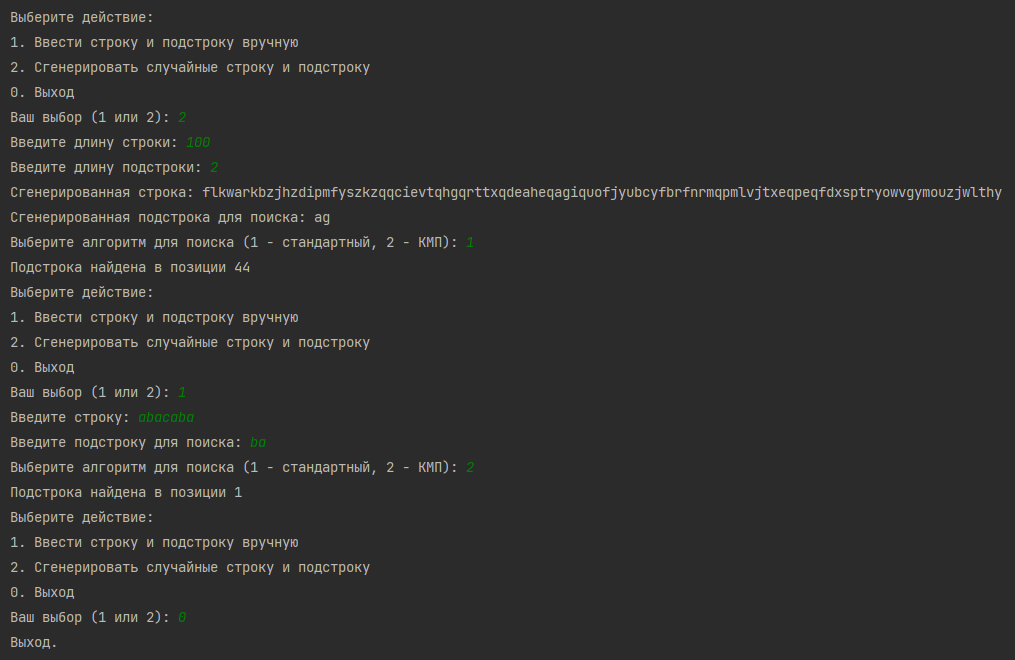
\includegraphics[width=1\linewidth]{images/example}
	\caption{Пример работы программы}
	\label{fig:example}
\end{figure}

\newpage

\subsection{Оценка числа сравнений алгоритмов}
Для обоснования, какой случай является худшим в текущей реализации алгоритмов: случай отсутствия подстроки длиной S или случай нахождения её в строке на последних S позициях, проведены соответствующие замеры.

Введём обозначения:
\begin{itemize}[]
	\item СБВ --- стандартный алгоритм без вхождения подстроки;
	\item КБВ --- алгоритм КМП без вхождения подстроки;
	\item СВН --- стандартный алгоритм с вхождением подстроки в начале текста;
	\item КВН --- алгоритм КМП с вхождением подстроки в начале текста;
	\item СВК --- стандартный алгоритм с вхождением подстроки в конце текста;
	\item КВК --- алгоритм КМП с вхождением подстроки в конце текста.
\end{itemize}

В таблице~\ref{tab:comp} приведены усредненные значения кол-ва сравнений за время работы алгоритмов в 1000 испытаниях.

\begin{table}[hbtp]
	\centering
	\caption{Число сравнений}
	\label{tab:comp}
	\csvreader[
%	head=false,
	tabular=|r|r|r|r|r|r|r|r|,
	table head=\hline Длина текста & Длина подстроки & СБВ & КБВ & СВН & КВН & СВК & КВК \\ \hline,
	late after last line=\\\hline,
	]{../src/lab_07/results_comparison.csv}{}{\csvlinetotablerow}
\end{table}

Соответствующий таблице график приведён на рисунке~\ref{fig:comp}
\begin{figure}
	\centering
	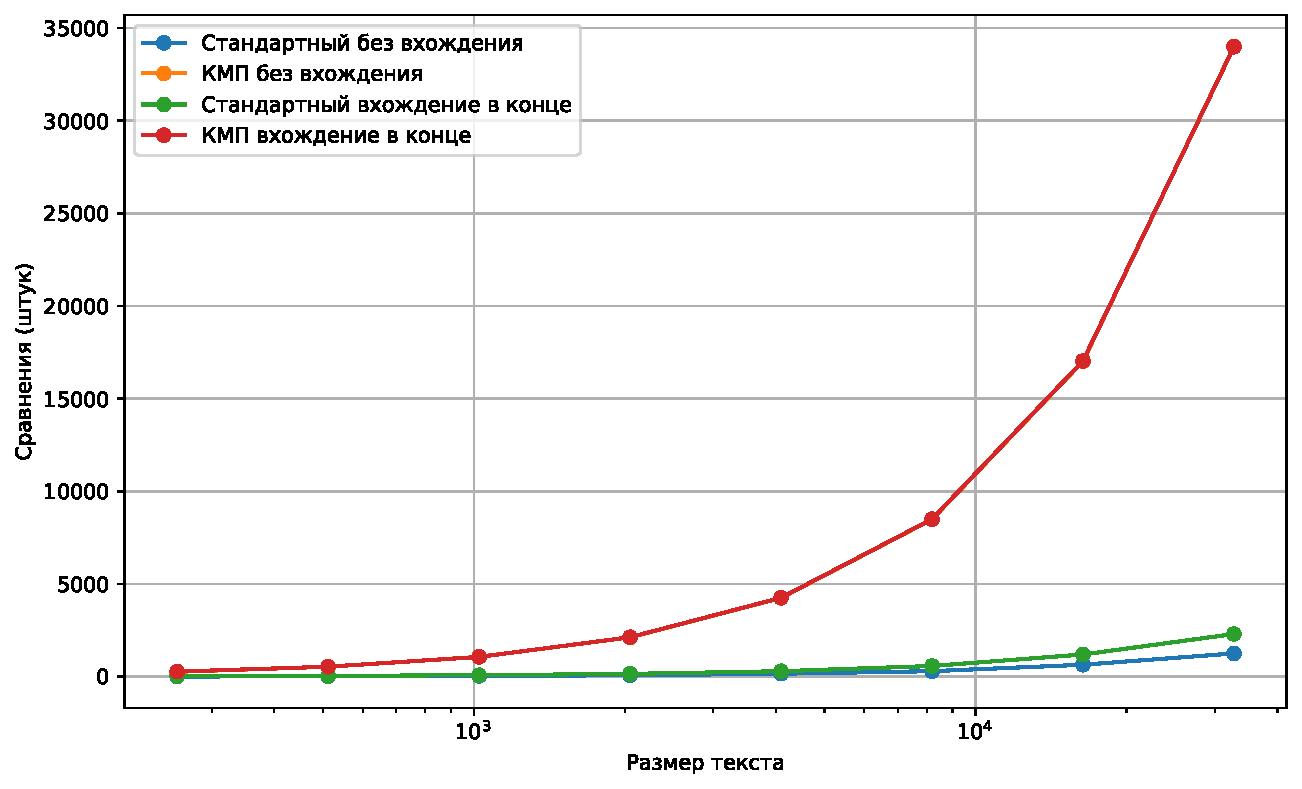
\includegraphics[width=1\linewidth]{../src/lab_07/results_comparison_logscale}
	\caption{Количество сравнений алгоритмов}
	\label{fig:comp}
\end{figure}

Стандартный алгоритм производит больше сравнений, если подстрока присутствует в конце текста, нежели если её нет в тексте вовсе.
То же самое нельзя сказать про КМП --- по результатам замеров кол-во сравнений при присутствии подстроки в тексте было больше кол-ва сравнений при втором случае в $\dfrac{3}{8}$ случаях.
Причем зависит это от того, какой текст был сгенерирован: в случае большого кол-ва совпадений префиксов подстроки с множеством подстрок текста значения в масиве префиксов больше.
Следовательно, сдвиги будут больше, а кол-во сравнений --- меньше.

\subsection{Время выполнения реализованных алгоритмов}
Функция perf\_counter из библиотеки time~\cite{time} возвращает время в секундах --- значение типа float.
Является самым точным методом замера коротких промежутков времени~\cite{perf}.

Результаты средних значений 1000 измерений времени работы алгоритмов приведены на рисунке \ref{fig:results}.
\begin{figure}
	\centering
	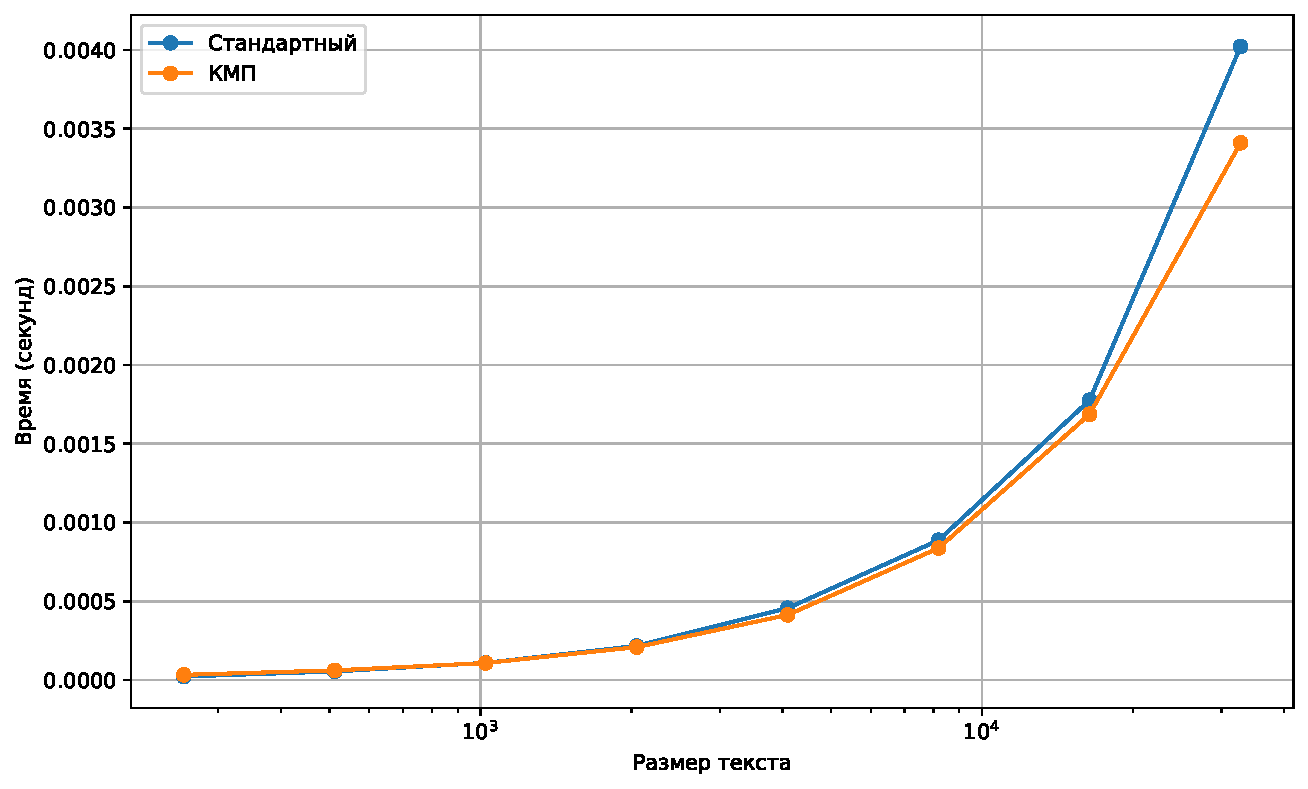
\includegraphics[width=1\linewidth]{../src/lab_07/results_logscale}
	\caption{Время выполнения алгоритмов}
	\label{fig:results}
\end{figure}

%Начиная с размера текста 1000, стандартный алгоритм выполняется дольше, чем алгоритм КМП.

\subsection*{Вывод}
В случае отсутствия подстроки в тексте кол-во сравнений стандартного алгоритма не превышает кол-во сравнений в случае, когда строка находится в конце.

Количество сравнений в случае нахождения подстроки в конце текста и её отсутствия для алгоритма КМП практически одинаково.

При размере текста в 256 символов стандартный алгоритм быстрее алгоритма КМП на 30\%.
Далее, до 1000 символов разница во времени между стандартным алгоритмом и КМП меньше 11\%.
Для текстов длиннее 1000 символов рекомендуется использовать алгоритм КМП, т.к. по мере увеличения длины исходной строки время поиска подстроки алгоритмом КМП будет расти медленнее, чем время при поиске стандартным алгоритмом.
Соответственно, чем больший размер текста --- тем больший выигрышь даёт алгоритм КМП.
При тексте в 32768 символов алгоритм КМП работает на 11\% быстрее, чем стандартный.
